% Chapter 1

\chapter{Introducción} % Chapter title

\label{ch:introduccion} % For referencing the chapter elsewhere, use \autoref{ch:introduccion}
\lhead{\emph{Introducción}} % Change X to a consecutive number; this is for the header on each page - perhaps a shortened title

%----------------------------------------------------------------------------------------
En este capítulo se introduce brevemente la problemática a resolver así como la estructura de la tesis.

En la Sección \ref{sc:definitions} se introducen la definiciones previas, necesarias, para el desarrollo de la tesis, utilizadas
luego como conocimientos de base, necesarias para poder comprender el trabajo en su totalidad.

En la Sección \ref{sc:context} se introduce el contexto del problema, para poder comprender el marco de área de estudio
propuesto, el tipo de antena objeto de estudio, los tipos de calibración y la importancia de la calibración interna.

En la Sección \ref{sc:motivation} se introduce cuál es la motivación para la realización de la presente tesis. Se hace foco
en la calibración interna clásica, sus virtudes y defectos y la necesidad de resolver problemas que la calibración clásica no
resuelve. Existen diversos métodos pero en todos se propone la incorporación de hardware externo adicional lo cual en algunos 
casos puede ser no implementable.

En la Sección \ref{sc:objective} se introduce el Objeto de la Tesis. En primera instancia se propone un método para 
complementar el método clásico de calibración interna sin necesidad de tener que agregar hardware externo, con todas las 
desventajas del caso desde el punto de vista de recursos y confiabilidad. En segunda instancia se proponen y listan todos los 
puntos a desarrollar a lo largo de esta tesis. Por ejemplo, el desarrollo de un modelo de base en RF sobre el cual evaluar la 
propuesta.

En la Sección \ref{sc:specifications} se introducen las Especificaciones del Problema. Es decir, las hipótesis de base que se
toman como necesarias para poder implementar el método propuesto.

En la Sección \ref{sc:methodology}, se explica la metodología utilizada a lo largo del proceso de desarrollo de la tesis.

En la sección \ref{sc:contribution} se introduce la contribución del presente trabajo de tesis a la comunidad científica.

En la sección \ref{sc:structure}, se introduce la Estructura de la tesis, en donde se detallan los capítulos de la tesis y su
contenido.


\section{Definiciones previas} \label{sc:definitions}

A continuación se introducen algunas definiciones previas necesarias para el desarrollo de la tesis. Las mismas se encuentran ordenadas de manera tal que la definición en cual se basa posea las bases ya mencionadas.
\todo{informar el orden de aparicion de las definiciones}

{\textbf{Antena:}} Es definida como la estructura transicional enre espacio libre y un dispositivo guía, como se muestra en la 
figura \ref{fig:antenna}. El dispositivo guía o línea de transmisión puede ser un cable coaxial o un tubo hueco (guía de 
onda), el cual es utilizado para transportar energía electromagnética desde la fuente de transmisión a la antena, o deade la 
antena al receptor. En el primer caso sería una configuración de antena transmisora y en el segundo, receptora \cite{Balanis2012}.
\begin{figure}[H]
 \centering
 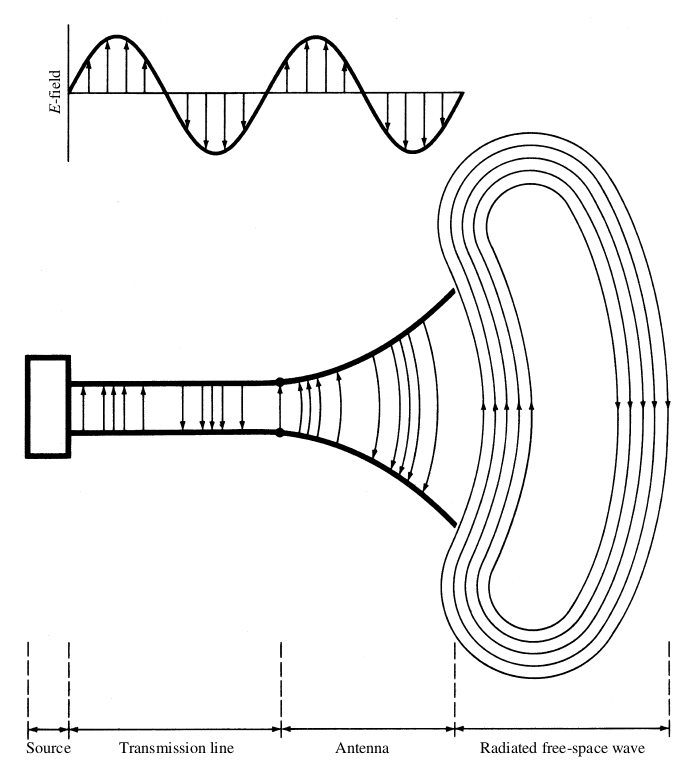
\includegraphics[width=10cm]{gfx/antenna.png}
 \caption{Antena como un dispositivo de transmisión \cite{Balanis2012}.}
 \label{fig:antenna}
\end{figure}

Hay una amplia variedad de antenas en la actualidad, en la tabla \ref{tab:type_antennas} se puede observar una agrupación 
simplificada.

\begin{table}[H]
  \footnotesize
  \centering
  \begin{tabular}{|c|p{9cm}|}
	\hline
	\textbf{Tipo Antena} & \textbf{Características} \\\hline
	Isotrópica & Es una antena hipotética, la cual radia la misma potencia en todas las direcciones.\\\hline
	Monopolo & Es un único módulo radiante, generalmente un simple cilindro de metal conectado en una punta a un plano de
	tierra y en la otra a la línea de alimentación. Usos: Radio AM/FM, walkie talkie, etc. \\\hline
	Dipolo & Es el tipo de antena más comúnmente utilizada, consiste en dos RMs simétricos, los cuales son cilindros
	metálicos o cables. Usos: antena de canales de tv VHF, antena de televisión analógica, etc. \\\hline
	Conjunto & Consiste en múltiples antenas trabajando como una única antena. Usos: Transmisión de canales de tv en VHF,
	detección de misiles, comunicaciones satelitales, etc.\\\hline
	Lazo & Consiste en una o múltiples vueltas de cable. Trabajan con campos magnéticos en vez de eléctricos. Usos: receptora
	de canales UHF de tv, receptoras de radio de Amplitud Modulada, etc.\\\hline
	Apertura & Son el principal tipo de antenas direccionales utilizadas en frecuencias microondas. Consisten en una antena
	del tipo dipolo o Lazo junto a una estructura que guía las ondas en una dirección determinada. Usos: Comunicaciones
	satelitales, comunicaciones marinas, etc.\\\hline
  \end{tabular}
  \caption{Características de cada grupo principal de antenas}
  \label{tab:type_antennas}
\end{table}


En el caso de esta tesis, se tiene un conjunto de antenas individuales, denominadas elementos radiantes (ER), que se usan tanto
para recibir como para transmitir. Dicho conjunto forma una red de difraccion que es el arreglo en fase, explicado más adelante.

{\textbf{Polarización:}} La polarización de una onda radiada se la define como la propiedad de una onda electromagnética 
describiendo la variación en tiempo de la dirección y la magnitud relativa del vector del campo eléctrico; específicamente, 
la figura trazada en funcion del tiempo por la extremidad del vector en un lugar fijo en el espacio, y el sentido en que es
trazado, como observado a lo largo de la dirección de propagación. Por lo tanto, la polarización es la curva trazada por la
punta del vector que representa el campo eléctrico instantáneo \cite{Balanis2012}. 

La polarización se puede clasificar como lineal, circular o elíptica (ver figura \ref{fig:hvPolarizations}). Si el vector que 
describe el campo eléctrico en un punto del espacio en función del tiempo recorre un trayecto a lo largo de una línea, se dice
que el campo es polarizado linealmente (horizontalmente o verticalmente). En general, la figura trazada por el campo eléctrico 
es una elipse, nombrada polarización elíptica. La polarización lineal y circular son casos especiales de la elíptica \cite{Vita2012}.

\begin{figure}[H]
 \centering
 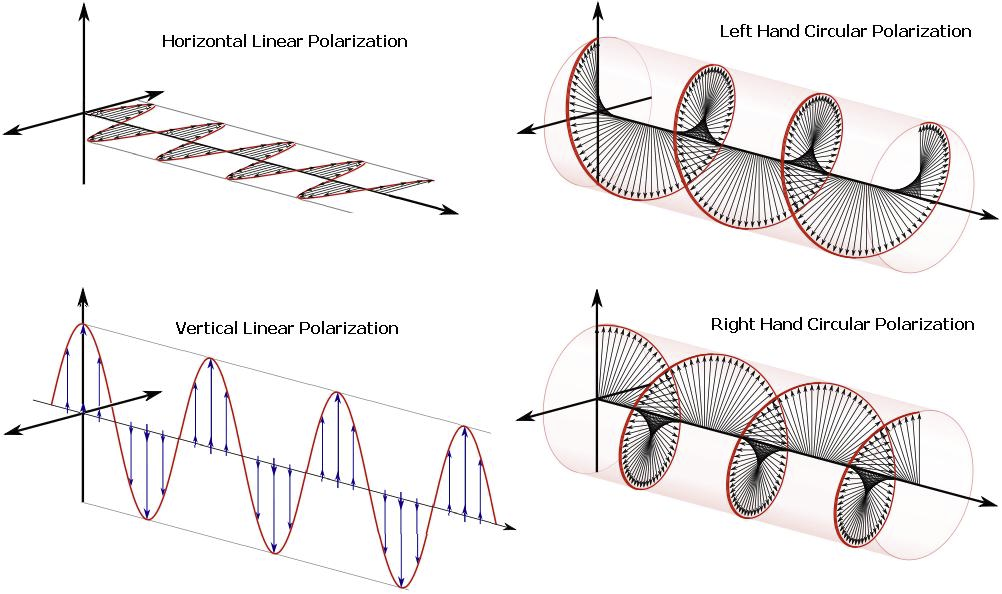
\includegraphics[width=10cm]{gfx/polarizations.png}
 \caption{Distintos tipos de polarizaciones \cite{Vita2012}}
 \label{fig:hvPolarizations}
\end{figure}

Para el caso de esta tesis, los elementos radiantes se consideran que tienen fase lineal, con una componente Horizonal (H) y una
componente Vertical (V), cada elemento radiante (ER) puede transmitir y recibir respectivamente.

{\textbf{Diagrama de radiación (del inglés: array pattern):}} Es una función matemática o una representación gráfica de las propiedades de radiación de
una antena en función de las coordenadas de espacio. En general es determinado en la región de campo lejano en función de las
coordenadas direccionales. Las propiedades de radiación incluyen el flujo de la densidad de potencia, intensidad de radiación,
fuerza del campo, directividad y fase o polarización \cite{Balanis2012}.

\todo{Fran: acá debajo poné por favor un diagrama de radiación de un arreglo en fase con cortes verticales (o en RANGO) y horizontales (o en AZIMUTH).}

\begin{figure}[H]
 \centering
 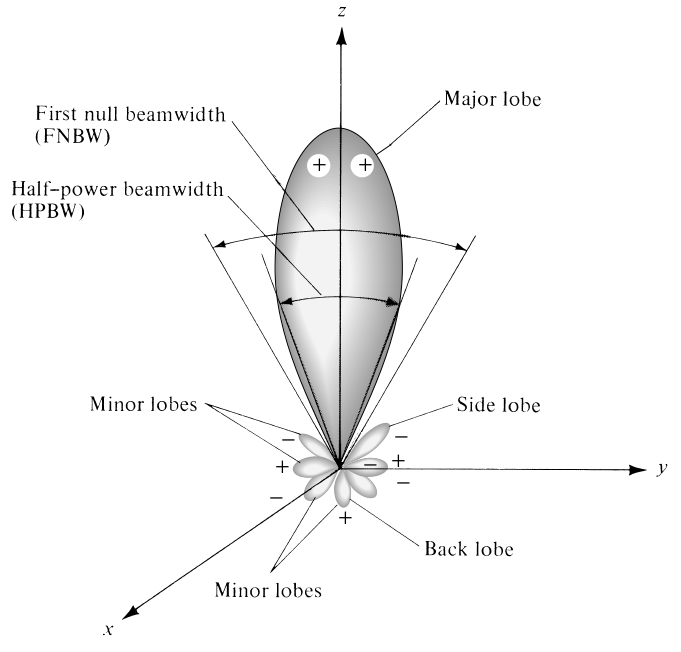
\includegraphics[width=10cm]{gfx/arrayPattern.png}
 \caption{Ejemplo de diagrama de radiación \cite{Balanis2012}.}
\end{figure}

En el caso de esta tesis, los diagramas de radiación son los típicos de un arreglo en fase, con un lóbulo principal, vinculado
al apuntamiento, y lóbulos secundarios.

{\textbf{Apuntamiento del haz:}} Es cambiar la dirección del lóbulo principal del diagrama de radiación. Puede ser realizada 
modificando la fase relativa entre los elementos radiantes de un conjunto de antena \cite{Standard1996}. En la siguiente figura 
se muestran diferentes apuntamientos que se pueden hacer con una antena de arreglo en fase. \todo{(agregar la figura)}

\todo{Fran: aca hace falta un dibujo en el que se muestra que desde un control electronico central se comanda elecfronicamente cada uno de los transmisores y receptores y con ello el apuntamiento total.  Por ende, se trata de un sistema controlado desde un sistema de control electronico central que define las fases y atenuaciones de cada uno de los elementos radiantes.}

{\textbf{Huella:}} Si se utiliza una antena de arreglo en fase apuntando hacia la tierra, montada en un dron, avión, satélite o
medio similar, la huella es la traza representada por la intersección del lobulo principal con la tierra. 

\todo{Fran: pone debajo una imágen aclarando.}

En el caso de esta tesis, si la antena se utiliza en alguno de los medios mencionados, es el resultado del apuntamiento sobre la
tierra, sobre la zona que se desea barrer. De esta forma, por ejemplo, un error de apuntamiento implicaría no estar visualizando
la zona que se desea \enquote*{ver}.

{\textbf{Parámetros S:}} La sigla S deriva de la palabra dispersión. Para altas frecuencias, es conveniente describir una
determinada red en términos de ondas en vez de tensiones o corrientes. Esto permite una definición más sencilla de planos
de referencia. Por razones prácticas, la descripción en términos de ondas entrantes y salientes ha sido introducida. Ahora,
una red de 4 polos se transforma en 2 puertos y $2n$ polos se transforman en $n$ puertos. En el caso de un número impar de polos
(ej. 3 polos), un punto de referencia puede ser elegido, atribuyendo un polo igualmente a dos puertos. Por lo tanto 3 polos se
convierten en 3 + 1 polo correspondiendo a 2 puertos. Como una regla general, para cantidades impares de polos, siempre se agrega
un polo extra.

\begin{figure}[H]
 \centering
 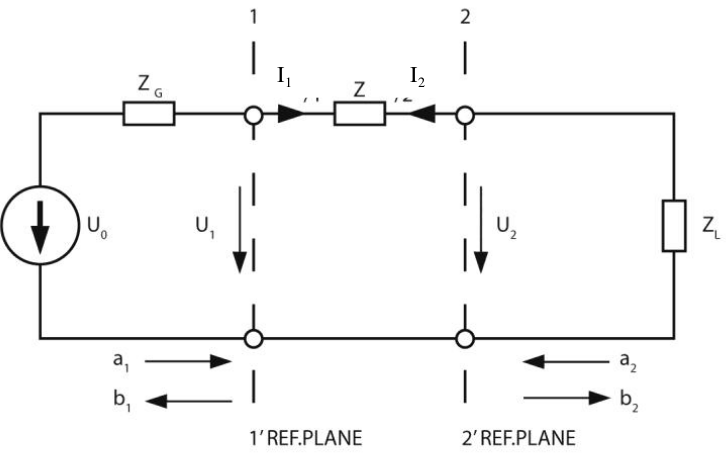
\includegraphics[width=10cm]{gfx/sParameters1.png}
 \caption{Ejemplo de una red de 2 puertos: circuito serie}
 \label{fig:esquema_serie}
\end{figure}

Tomando como ejemplo una red de 2 puertos compuesta por una sola impedancia $Z$ conectada en serie (\ref{fig:esquema_serie}).
Las impedancias de la fuente y de la carga son $Z_G$ y $Z_L$ respectivamente. Si $Z=0$ y $Z_L = Z_G$ (para el caso de $Z_G$ real)
la carga está adaptada. En este caso se obtiene una máxima transferencia de potencia y $U_1 = U_2 = U_0/2$. Notar que todas las
tensiones y corrientes son valores pico. Se supone que las líneas que unen los componentes poseen longitud eléctrica igual a 0.
Las conexiones con una longitud eléctrica finita están dibujadas como una doble línea. A continuación se relacionará $U_0$, $U_1$
y $U_2$ a $a$ y $b$.


\subsection{Definición de \enquote*{ondas de potencia}}

Las ondas incidentes al puerto son $\textbf{a}=(a_1, a_2, a_3, ..., a_n)$, las ondas salientes, o reflejadas, del puerto son
$\textbf{b}=(b_1, b_2, b_3, ..., b_n)$. Por definición, las corrientes incidentes son positivas y las salientes negativas. La
onda $a_1$, incidente al puerto 1, es derivada de la tensión entrante a la carga balanceada.

Para hacer qe esta definición sea consistente con la ley de la conservación de la energía. La tensión es normalizada a $\sqrt{Z_0}$.
$Z_0$ es, en general una impedancia de referencia arbitraria, que usualmente se la utiliza como la impedancia característica de la
línea (ej, $Z_0 = 50 \Omega$). Y, cuando todas las impedancias son iguales ($Z_G = Z_L = Z_0$), se dice que la línea está adaptada
y no hay onda reflejada. Las definiciones de $a1$ y $b1$ son:

\begin{equation}
\begin{aligned}
	a1 &= \dfrac{U_0}{2\sqrt{Z_0}}= \dfrac{\textrm{onda de tensión incidente (puerto 1)}}{\sqrt{Z_0}}=\dfrac{U_1^{inc}}{\sqrt{Z_0}} \\
	b1 &= \dfrac{U_1^{refl}}{2\sqrt{Z_0}}= \dfrac{\textrm{onda de tensión reflejada (puerto 1)}}{\sqrt{Z_0}}
\end{aligned}
\end{equation}

Notar que \textbf{a} y \textbf{b} tienen las unidades de $\sqrt{\textrm{potencia}}$.

La potencia incidente al puerto 1, $P_{inc}$, es simplemente la potencia entregada por la fuente, mientras que la potencia saliente
del puerto 1, $P_{refl}$, viene de la onda de tensión reflejada.

\begin{equation}
\begin{aligned}
	P_1^{inc} &= \dfrac{1}{2}|a_1|^2= \dfrac{|U_1^{inc}|^2}{2Z_0}=\dfrac{|I_1^{inc}|^2}{2}Z_0 \\
	P_1^{refl} &= \dfrac{1}{2}|b_1|^2= \dfrac{|U_1^{refl}|^2}{2Z_0}=\dfrac{|I_1^{refl}|^2}{2}Z_0 \\
\end{aligned}
\end{equation}

En el caso de una desadaptación de la impedancia de carga $Z_L$, parte de la potencia será reflejada a través del puerto 2 (
potencia incidente al puerto 2).

$$
P_2^{inc}=\dfrac{1}{2}|a_2|^2
$$

Se ha definido $a_1 = U_0/2\sqrt{Z_0} = U^{inc}/\sqrt{Z_0}$ con la onda de tensión incidente $U^{inc}$. Como analogía
se la puede definir como $a_1 = I^{inc}\sqrt{Z_0}$ con la onda incidente de corriente $I^{inc}$. Utilizando ambas, se obtiene la
definición general de las ondas incidentes $a_i$ y reflejadas $b_i$ de un puerto.

\begin{equation}
\begin{aligned}
	a_i &= \dfrac{U_i + I_iZ_0}{2\sqrt{Z_0}} \\
	b_i &= \dfrac{U_i - I_iZ_0}{2\sqrt{Z_0}}
\end{aligned}
\label{eq:waves}
\end{equation}

Solucionando este sistema de ecuaciones, $U_i$ y $I_i$ pueden ser obtenidas de $a_i$ y $b_i$ como

\begin{equation}
\begin{aligned}
	U_i &= \sqrt{Z_0}(a_i + b_i) = U_i^{inc} + U_i^{refl}\\
	I_i &= \dfrac{1}{\sqrt{Z_0}}(a_i - b_i) = \dfrac{U_i^{refl}}{Z_0}
\end{aligned}
\end{equation}


\subsection{La matríz de parámetros S}

La relación entre $a_i$ y $b_i$ (siendo $i=1..n$) puede ser escrito como un sistema de n ecuaciones lineales (siendo la variable
independiente $a_i$ y $b_i$ como la dependiente)

\begin{equation}
\begin{aligned}
	b_1 = S_{11}a_1 + S_{12}a_2 \\
	b_2 = S_{21}a_1 + S_{22}a_2
\end{aligned}
\label{eq:s_matrix}
\end{equation}

Escrito de forma matricial: \textbf{b} = \textbf{Sa}

El significado físico de los parámetros S son los siguientes:
\begin{itemize}
	\item $S_{11}$: es el coeficiente de reflexión con la salida de la red terminada en una carga adaptada ($a_2 = 0$).
	\item $S_{21}$: es la transmisión en directa (del puerto 1 al 2)
	\item $S_{12}$: es la transmisión en inversa (del puerto 2 al 1)
	\item $S_{22}$: es el coeficiente de reflexión de la salida.
\end{itemize}

Al medir todos los parámetros S de una red de n puertos, todos los puertos deben estar terminados con una carga adaptada.
Utilizando las equaciones \ref{eq:waves} y \ref{eq:s_matrix} se obtiene el coeficiente de reflexión de una impedancia $Z_L$
conectada a un generador de impedancia de salida $Z_0$ (Figura \ref{fig:esquema_serie}, caso $Z_G = Z_0$ y $Z = 0$):

\begin{equation}
S_{11} = \dfrac{b_1}{a_1}\bigg|_{a_2=0} = \dfrac{U_1 - I_1Z_0}{U_1 + I_1Z_0} = \dfrac{Z_L - Z_0}{Z_L + Z_0} = \Gamma
\end{equation}


\subsection{La matriz de transferencia} \label{ssec:transMatrix}

Resulta muy conveniente la utilización de la matriz de parámetros S para describir una red de n polos en términos de ondas y
para mediciones. Pero, no es muy conveniente su utilización para caracterizar la respuesta de una cascada de redes de 2
puertos. En este caso, una manera de encarar dicha problemática, es la utilización de la matriz de parámetros T (matriz
de transferencia), la cual relaciona las ondas de entrada y salida de cada cuadripolo.

\begin{equation}
\begin{pmatrix} a_1\\b_1 \end{pmatrix} = \begin{pmatrix} T_{11} & T_{12}\\T_{21} & T_{22} \end{pmatrix}
\begin{pmatrix} a_2\\b_2 \end{pmatrix}
\end{equation}

Cabe destacar que, para los casos en que no hay transmisión entre el puerto 1 y 2, si bien la matriz de parámetros S está definida,
la matriz de parámetros T no. La matriz resultante de parámetros T de una cascada de redes de 2 puertos resulta como sigue:

\begin{equation}
\mathbf{T_M=T_1T_2...T_m}
\label{eq:cascade}
\end{equation}

\subsection{Conversión entre parámetros T y S} \label{ssec:conversion}

Como la matriz de transferencia (T) simplemente relaciona las ondas de entrada y salidas de una forma diferente a la matriz de
scattering, partiendo de una matriz se puede llegar a la otra y viceversa.

\begin{equation}
	\begin{aligned}
		T_{11} &= S_{12} - \dfrac{S_{22}S_{11}}{S_{21}},\quad T_{12} = \dfrac{S_{11}}{S_{21}} \\
		T_{21} &= - \dfrac{S_{22}}{S_{21}},\qquad\qquad T_{22} = \dfrac{1}{S_{21}}
	\end{aligned}
	\label{eq:s2t}
\end{equation}

Para obtener los parámetros S partiendo desde los parámetros T, se utiliza la siguiente relación matemática

\begin{equation}
	\begin{aligned}
		S_{11} &= \dfrac{T_{12}}{T_{22}},\qquad S_{12} = T_{11} - \dfrac{T_{12}T_{21}}{T_{22}} \\
		S_{21} &= \dfrac{1}{T_{22}},\qquad S_{22} = - \dfrac{T_{21}}{T_{22}}
	\end{aligned}
	\label{eq:t2s}
\end{equation}


\subsection{Propiedades de la matriz de parámetros S}

Una red generalizada de n puertos posee $n^2$ coeficientes de dispersión. Mientras que los $S_{ij}$ podrían ser todos independientes,
en general, debido a simetrías u otros factores, la cantidad de coeficientes independientes es mucho menor.
\begin{itemize}
	\item Una red de n puertos es recíproca cuando $S_{ij} = S_{ji}$ para todo $i, j$. La mayoría de los componentes pasivos son
		recíprocos (resistencias, capacitores, transformadores, etc., exceptuando para estructuras involucrando ferrites magnéticos,
		plasmas, etc.), componentes activos como amplificadores generalmente son no recíprocos.
	\item Una red de 2 puertos es simétrica cuando es recíproca ($S_{21} = S_{12}$) y cuando los coeficientes de reflexión son iguales
		($S_{11} = S_{22}$).
	\item Una red de N puertos es pasiva y sin pérdidas si su matriz de parámetros S es unitaria ($\mathbf{S^{\dagger}S = 1}$ donde
		$\mathbf{x^{\dagger} = (x^*)^T}$ es la conjugada y transpuesta de $x$). Para una red de 2 puertos esto significa

\begin{equation}
S^{\dagger}S = \begin{pmatrix} S_{11}^* & S_{21}^*\\S_{12}^* & S_{22}^* \end{pmatrix}
			\begin{pmatrix} S_{11} & S_{12}\\S_{21} & S_{22} \end{pmatrix} = \begin{pmatrix} 1 & 0\\0 & 1 \end{pmatrix}
\end{equation}

Esto conlleva a 3 condiciones

\begin{equation}
\begin{aligned}
	|S_{11}|^2 + |S_{21}|^2 = 1 \\
	|S_{12}|^2 + |S_{22}|^2 = 1 \\
	S_{11}^*S_{12} + S_{21}^*S_{22} = 0
\end{aligned}
\label{eq:sCondition}
\end{equation}

Separando la última ecuación en módulo y fase, se obtiene

\begin{equation}
\begin{aligned}
	|S_{11}||S_{12}| &= |S_{21}||S_{22}| \\
	-argS_{11} + argS_{12} &= -argS_{21} + argS_{22} + \pi
\end{aligned}
\label{eq:con}
\end{equation}

Donde $arg(x)$ es el argumento (ángulo) de la variable compleja $x$. Combinando la ecuación \ref{eq:sCondition} con la primera
de la ecuación \ref{eq:con} se obtiene

\begin{equation}
\begin{aligned}
	|S_{11}| = |S_{12}|, |S_{21}| = |S_{22}| \\
	|S_{11}| = \sqrt{1 - |S_{12}|^2}
\end{aligned}
\end{equation}

Por lo tanto, cualquier red de 2 puertos sin pérdidas puede ser caracterizada con un módulo y tres ángulos.
\end{itemize}

En general los parámetros S son valores complejos y dependientes de la frecuencia.
{\textbf{Analizador de espectro vectorial o VNA:}} Es un instrumento que mide los parámetros eléctricos de una red. Hoy, dichos
analizadores miden los parámetros S porque las reflexiones y transmisiones de redes eléctricas son fácilmente medibles en alta
frecuencia. Normalmente caracterizan redes de dos puertos \cite{NetworkAnalyzer}.

En esta tesis se utiliza el mismo concepto que utiliza un VNA para determinar los parámetros S en los diferentes lazos de 
calibración.

{\textbf{Directividad:}} Es una figura de mérito de una antena. Es el cociente entre la densidad de potencia radiada en la
dirección de máxima emisión y la densidad de potencia radiada utilizando un radiador isotrópico, el cual emite uniformemente
en toda dirección \cite{Standard1996}.

El concepto de directividad se utiliza en esta tesis al explicar y analizar los lazos de calibración.

{\textbf{Relación de onda estacionaria (del inglés SWR):}} Es una medida de adaptación entre la carga y la impedancia
característica de una línea de transmisión. Las desadaptaciones de impedancias resultan en ondas estacionarias a lo largo de
dicha línea de transmisión. El SWR está definido como la relación entre la amplitud de la onda reflejada y la amplitud de la
onda incidente \cite{swrWiki}.

En el caso de esta tesis, se incluyen los efectos de desadaptación de impedancias dentro del modelo construido para evaluar el
algoritmo de calibración propuesto.

{\textbf{Adaptación de impedancias:}} La máxima transferencia de potencia requiere que la impedancia de un sistema de
antena esté adaptada al complejo conjugado de la impedancia del transmisor o receptor. En el caso de un transmisor,
la impedancia adaptada deseada no necesariamente corresponde a la impedancia de salida dinámica del transmisor analizado
como una impedancia sino al valor de diseño (típicamente de $50 \Omega$) requerido para una operación eficiente
y segura del circuito de transmisión. Normalmente, la impedancia deseada es resistiva pero un transmisor (y algunos receptores)
pueden tener ajustes adicionales para cancelar una cierta cantidad de reactancia en orden de obtener dicha adaptación. Cuando
una línea de transmisión es utilizada entre la antena y el transmisor (o receptor) uno generalmente desearía un sistema de antena
con una impedancia resistiva cercana a la impedancia característica de dicha línea de transmisión, para minimizar el SWR
e incrementar la transmisión \cite{AntennaWiki}.

En el caso de esta tesis, en el modelo físico desarrollado se tiene en cuenta la posibilidad de incorporar desadaptaciones.

{\textbf{Conjunto de Antena con fase variable (en inglés: Phased Array):}} es un conjunto de antenas en que las fases relativas
de las señales con que se alimenta cada antena se varían intencionalmente con objeto de alterar el diagrama de radiación del
conjunto. Normalmente se refuerza la radiación en una dirección concreta y se suprime en direcciones indeseadas. Si todos los
elementos del conjunto están contenidos en el mismo plano y la señal con que se alimentan es de la misma fase,
entonces se estará reforzando la dirección perpendicular a ese plano. Si se altera la fase relativa de las señales se podrá
\enquote*{direccionar el haz} de modo que las interferencias resulten constructivas. Se consigue de este modo hacer barridos sin
necesidad de movimiento físico, mecánico, con la ventaja añadida de que se pueden barrer ángulos del orden de miles de grados
por segundo. Esto permite utilizar la antena para compaginar simultáneamente funciones de detección y de seguimiento de blancos
individuales, así como para obtener imágenes de apertura sintética, para el caso en que el arreglo de antenas con fase se 
utilice con dicho propósito. Su uso se va extendiendo debido a la confiabilidad derivada del hecho de que no posee partes
móviles. Casi todos los radares militares modernos se basan en conjuntos de antenas, relegando los sistemas basados en antenas
rotatorias a aplicaciones donde el costo es un factor determinante (tráfico aéreo, meteorología) Su uso está también 
extendido en aeronaves militares debido a su capacidad de seguir múltiples objetivos. El primer avión en usar uno fue el B-1B
Lancer, y el primer caza, el MiG-31 ruso.\\
\todo{buscar referencia y poner 2 imagenes sin satelites, drone con radar y solo radar}

Para esta tesis se analizan dos antenas de este tipo:.. (y acá agregar las dimensiones y las caraceristicas resumidas de las antenas que se analizan..)
\todo{completar lo anteriormente dicho}

{\textbf{Calibración:}} La calibración es el proceso de comparar los valores obtenidos por un instrumento de medición con la
medida correspondiente de un patrón de referencia o estándar. Según la Oficina Internacional de Pesas y Medidas, la 
calibración es \enquote*{una operación que, bajo condiciones específicas, establece en una primera etapa una relación entre
los valores y las incertidumbres de medida provistas por estándares e indicaciones correspondientes con las incertidumbres de 
medida asociadas y, en un segundo paso, usa esta información para establecer una relación para obtener un resultado de la 
medida a partir de una indicación}.

Para el caso particular de esta tesis, y de este tipo de antenas, la calibración permite conocer y controlar con cierta 
exactitud conocida el apuntamiento de la antena. En terminos generales puede clasificarse la calibracion en externa e interna. 
\begin{itemize}
	\item La calibración externa requiere del uso de una masa patrón externa. Durante una calibración externa, la calibración se
		ajusta con respecto a las constantes de la masa patrón externa. 
	\item La calibración interna no requiere de un patrón externo. Con la calibración interna, las constantes de calibración de
		la antena se ajustan con respecto a referencias precisas existentes en la misma antena.
\end{itemize}

{\textbf{Calibración interna de un conjunto de antena:}} Las mediciones obtenidas utilizando este sistema son útiles solamente
al utilizarlas en conjunto a los resultados de los test realizados en tierra, los cuales definen la relación entre lo observado
y la performance de los parámetros del sistema. Ejemplos de este tipo de antenas para los cuales se utilizó calibración 
interna son el E-ERS-1 y el SIR-C.

Los tests realizados en tierra, para dichos sistemas complejos, son sobre la electrónica de RF, la electrónica digital y la
antena en temperatura; para los cuales es preferible realizarlos, cuando sea posible, en un ambiente al vacío. Los
parámetros clave del sistema que son medidos en función de la temperatura para cada configuración de ganacia y PRF del radar
son: potencia transmitida, pérdidas de transmisión/recepción, ganancia de recepción, ganancia y diagrama de radiación de la 
antena, linealidad de la electrónica digital/RF, rango dinámico, y fase/amplitud vs estabilidad de la frecuencia. Los
elementos de calibración, como medidores de temperatura, de corriente y de potencia, podrán permitir la determinación del 
modelo en RF y la respuesta del sistema en función de la variación de dichos parámetros.

Esta técnica asume que la variación en la respuesta del sistema puede ser modelada en función de los parámetros observables.
También, se asume que los componentes de calibración están correctamente calibrados y son estables en el paso del tiempo.
Además de estos tests, en la mayoría de los sistemas de radar se realizan mediciones de componentes de RF utilizando lazos de
calibración \cite{Curlander1991}.

Para el caso particular de esta tesis, se calibrará la antena en RF utilizando el método clásico y el propuesto con 
acoplamientos mútuos.

{\textbf{Caracterización:}} significa medir (el desempeño de) los parámetros de un dispositivo con el objeto de describir en
forma comprensible su comportamiento \cite{Mittermayer2007}.

Para el caso particular de esta tesis, es necesario tener caracterizados los componentes de una antena para poder modelizar el 
comportamiento de la misma.

{\textbf{Caracterización del sistema:}} adicionalmente incluye la determinación de las curvas de características basadas
en los modelos y en las mediciones indirectas de los parámetros, en el caso en que los parámetros no pueden ser medidos
en forma directa \cite{Mittermayer2007}.

{\textbf{Verificación:}} Proceso donde se confirma que existen entradas y especificaciones adecuadas para cualquier actividad,
y que los resultados de dichas actividades son correctas y consistentes con las especificaciones y entradas mencionadas 
previamente \cite{Division2009}.


{\textbf{Radar:}}

{\textbf{Radar:}}

{\textbf{Radar de apertura sintética:}}

{\textbf{Chirp:}}

{\textbf{Chirp réplica:}}
\todo{todooo}


\section{Contexto} \label{sc:context}

La presente tesis se enfoca en el tipo \enquote*{conjunto de antena de fase controlada de manera electrónica}, en inglés
\enquote*{phase array electronically controlled antenna}. Este tipo de antenas son ampliamente utilizadas en aplicaciones donde 
es necesario realizar apuntamientos en diferentes direcciones con altas velocidades. Por ejemplo, comunicaciones móviles 
\cite{Chen2012}, aéreas \cite{MHong1989} y espaciales \cite{Shimada1995}\cite{Makhoul2012}. En el capítulo \ref{ch:phasedArray}
se explica el principio de funcionamiento básico de dicho tipo de antena.

Para generar diversos productos, por ejemplo imágenes satelitales en radares SAR \cite{Freeman1992}, es necesario que la
antena se encuentre correctamente calibrada \cite{Luscombe1990}\cite{Seifert1996}\cite{Dall1994}. Como fue mencionado 
previamente, implica que las tolerancias de fase y amplitud se mantengan en el tiempo y/o sus valores sean bien conocidos para
cada elemento del conjunto. Desde el control central se puede estar definiendo determinada fase y atenuacion para cada elemento
radiante, pero si la antena no esta calibrada, lo que realmente se desea y lo que resulta efectivo, pueden no coincidir.

Un método de calibración en tierra para estas antenas es la de utilización de fuentes externas de campo lejano o cercano
\cite{Agrawal2003}. Sin embargo, en aplicaciones aéreas o espaciales, la utilización de dichas fuentes es impráctica o
difícil de implementar \cite{Aumann1989}. Para estos casos se utilizan esquemas de calibración externa e interna.

Hay dos grupos principales de calibración externa a saber,
\begin{itemize}
	\item Calibración utilizando blancos puntuales: Los blancos puntuales son dispositivos construidos por el hombre, generalmente
		corner reflectors, transponders, generadores de tono o receptores. Estos dispositivos son considerados blancos puntuales porque
		son mucho menores a la huella de una antena y el eco de la señal reflejada o emitida por los mismos poee mucha más intensidad
		que dicha área. Por último, cabe destacar que, dado que el reflejo es bien conocido, se puede deducir la potencia transmitida
		por la antena. 
	\item Calibración utilizando blancos distribuidos: Se refiere a la utilización de blancos naturales de gran área con 
		propiedades de dispersión homogéneas. Se utiliza la suposición que dichas propiedades son estables o que su variación es
		bien conocida.
\end{itemize}

El mayor problema de dichos esquemas de calibración es que el tiempo de revisita a dichos lugares de calibración en tierra es muy
grande y solo se puede calibrar la ganancia absoluta del conjunto de antena en su totalidad. Para disminuir el tiempo entre
calibraciones y para poder calibrar cada elemento del conjunto de forma individual surge diversos esquemas de calibración
interna.

El primer método a mencionar es el llamado método REV, el cual calibra de a un módulo radiante a la vez utilizando una
antena externa al panel como receptora. En el proceso de calibración se transmite de a un módulo radiante a la vez
y se va variando su fase hasta obtener la máxima potencia recibida. Repitiéndose el proceso para todos los elementos.

Otro método es el convencional (descripto en el capítulo \ref{ch:classicalCalibration}), el cual implementa lazos internos
para calibrar los caminos de transmisión y recepción de la antena de forma independiente \cite{Makhoul2012}
\cite{Luscombe1990}\cite{Seifert1996}\cite{Dall1994}\cite{Freeman1995}\cite{Bibby2003}\cite{Bast2003}\cite{Stove2004}
\cite{Srivastava1996}\cite{Wang2010}. Para ello, la señal de calibración recibida se la compara con la potencia transmitida,
obteniendo así, que dicha diferencia se corresponde con el desfasaje de potencia y fase de cada camino de transmisión/
recepción. Luego, se opta por caracterizar todos aquellos componentes que no pertenecen a ningún lazo de calibración
\cite{Freeman1995}. Este método presenta algunos inconvenientes. Por ejemplo se puede mencionar que los recursos necesarios
(tiempo, personal) durante la campaña de ensayos previa al lanzamiento impactan en todo el desarrollo de actividades,
o las consecuencias que puede traer el hecho que la caracterización no sea válida porque un determinado componente
envejece con el paso del tiempo.

En este contexto, se investiga y propone un método que permita reducir costos asociados a la calibración y por ende a los
proyectos:

\begin{enumerate}
    \item Evitando la necesidad de realizar caracterizaciones previas del conjunto de antena.
    \item Permitiendo conocer en tiempo real, y para el estado real de la antena, los valores reales de fase y amplitud en
		vuelo que transmite la antena, independientemente de su estado de envejecimiento.
\end{enumerate}

En este sentido se investiga y aprovecha el concepto acoplamiento mutuo inherente entre los módulos radiantes de la antena
\cite{Aumann1989}, pero de manera complementaria al enfoque tradicional. Este método calibra tanto los caminos de transmisión
como recepción a la vez, para ello, se transmite en una polarización y se recibe en otra de a un módulo radiante a la vez.
Una ventaja que tiene frente a los otros métodos realizados es que no sólo calibra la antena en su totalidad, sino también
sirve para determinar si hay módulos radiantes en mal funcionamiento o directamente inhabilitados.

\section{Motivación} \label{sc:motivation}

Para poder hacer un uso adecuado de un conjunto de antena es necesario conocer la fase y atenuación de cada uno de los elementos
del mismo, tanto cuando transmiten como cuando recibe. Sin embargo, si bien uno controla la fase y atenuación de cada elemento,
la RFDN no permite necesariamente asegurar que la fase y atenuación con que sale la señal sea realmente la deseada. Hay 
fenómenos de dispersión en la RFDN debidos a la temperatura que hacen que la fase deseada y la requerida sean diferentes 
\cite{Keizer2011}.

El método de calibración tradicional, por lazos de calibración internos, permite calibrar un conjunto de antena, aunque
presenta algunos defectos entre los cuales se incluyen:

\begin{enumerate}
    \item Como los lazos de calibración utilizados en el método no abarcan la totalidad de la antena, no es posible detectar el
		mal funcionamiento o directamente la inhabilitación de un elemento que esté fuera de los mismos. 
    \item Como existen elementos que quedan fuera del lazo de calibración interna, por ejemplo los circuladores, es necesario
		realizar caracterizaciones en tierra, lo cual implica un consumo de recursos de proyecto importantes. Además se debe 
		asumir que dicha caracterización será válida (o sea que no habrá envejecimiento de los mismo) durante toda la vida útil
		de la antena.
    \item Cada lazo de calibración no se interrelaciona con el resto haciendo que no se pueda disminuir el error de medición por
		multiplicidad de caminos.
\end{enumerate}

El conocimiento de dichas limitaciones llevan a investigar opciones superadoras, que den lugar a un método de calibración que 
permita ser complementario al tradicional. A su vez, es necesario desarrollar un modelo de antena polarimétrica para poder 
comparar el desempeño de cada algoritmo para distintos estados del comportamiento de los componentes que conforman dicha antena.

El método propuesto en esta tesis, denominado de \enquote*{diseño y calibración de una antena polarimétrica por 
acoplamientos mutuos}, toma la idea de mediciones por acoplamiento mutuo \cite{Agrawal2003}\cite{Shipley2000} \cite{Aumann1989}
\cite{Chen2012} para integrarla de manera complementaria al método tradicional sin necesidad de agregar hardware adicional. 
Además, se establecen los requerimientos electrónicos para poder implementarla. Para poder comparar el comportamiento y 
eficiencia de ambos métodos, se realiza un modelo de antena polarimétrica.


\section{Objetivo de la Tesis} \label{sc:objective}

La presente tesis tiene varios objetivos:

\begin{enumerate}
    \item Presentar conceptualmente el método tradicional de calibración interna de una antena polarimétrica. Como resultado
		de este estudio se resumen inconvenientes en su utilización, que tienen un impacto en los recursos necesarios para poder ser
		implementada. 
    \item Investigar, desarrollar y presentar conceptualmente un método alternativo de calibración interna que introduzca
		mejoras al método tradicional sin necesidad de introducir hardware adicional y con la premisa fundamental de
		reducir los costos asociados a las caracterizaciones que el método tradicional incluye. Introducir los
		requerimientos necesarios para poder implementarlo.
    \item Investigar e implementar el modelo de antena polarimétrico que será utilizado para poder comparar el 
		método tradicional y el alternativo. Dicho modelo debe representar el comportamiento en RF básico de las señales al 
		propagarse por el sistema.
    \item Implementar los sistemas de calibración interna tradicional y alternativo que actúen sobre el modelo de antena. 
    \item Sacar conclusiones respecto a los pros y contras del método propuesto, en particular en referencia al método
		tradicional, por medio de algunos parámetros objetivos como ser tiempo de calibración, caracterizaciones necesarias,
		incertidumbre de medición, entre otros.
\end{enumerate}


\section{Especificaciones del problema} \label{sc:specifications}

Para poder aplicar e implementar el método de acoplamientos mutuos se deben cumplir las siguientes hipótesis de base, que a su
vez son consideradas las especificaciones del problema.

\begin{enumerate}
    \item Modularización de los componentes de la antena: la antena debe estar compuesta por desfasadores, atenuadores, cables,
		divisores de potencia y elementos radiantes, que son los componentes que conforman, interconectados entre sí, la antena. Estos
		elementos deben ser modelizados de manera modular de forma de poder intercambiarlos entre sí para poder simular diferentes
		topologías.

	\item Modelización de los componentes en RF: se desea que el comportamiento del modelo de antena que se construye sea 
		representativo de su comportamiento en RF desde el punto de vista de los efectos sobre la señal de interés.

    \item Sistemas LTI: la aplicación deberá reproducir el comportamiento del sistema, el cual será lineal e invariante
		en el tiempo.

	\item Adaptación de impedancias: todos los componentes se encuentran perfectamente adaptados.

    \item Variabilidad para determinados componentes: se deben poder utilizar distintos divisores/combinadores de potencia.
		La diferencia entre ellos es la cantidad de puertos de salida/entrada.

    \item Dimensión de antena: se debe poder configurar la cantidad de elementos radiantes por columna y fila de la antena.
    \item Distancia entre elementos radiantes: Se debe poder configurar la distancia entre elementos radiantes.

    \item Configuración individual de componentes: Se debe poder configurar los atributos que afecten la modelización de cada
		componente de la antena; largo, atenuación y desfasaje por metro de cables.

    \item Modelizacion de dispersiones: se debe poder configurar las dispersiones en el comportamiento de cada componente de la
		antena de forma independiente.

    \item Introducción de elementos de control en el lazo de calibración: se deben poder configurar los atenuadores y
		defasadores a la hora de realizar la calibración.

    \item Calibración clásica: sa aplicación debe poder calibrar una antena polarimétrica con el método de calibración clásico.

    \item Calibración por acoplamientos mutuos: sa aplicación debe poder calibrar una antena polarimétrica con el método de
		calibración propuesto.

    \item Calibración de ganancia: la aplicación debe poder calibrar la ganancia de transmisión y recepción.

    \item Calibración de fase: la aplicación debe poder calibrar la fase de transmisión y recepción.

    \item Calibración en polarización horizontal: la aplicación debe poder calibrar en la polarización horizontal.
    \item Calibración en polarización vertical: la aplicación debe poder calibrar en la polarización vertical.
    \item Calibración en Tx: la aplicación debe poder calibrar en transmisión.
    \item Calibración en Rx: la aplicación debe poder calibrar en recepción.

    \item Calibración independiente del estado inicial: se debe poder alcanzar el estado de calibración deseado partiendo
		cualquier estado inicial en los desfasadores y atenuadores.

    \item Transmisión vs recepción por polarizaciones cruzadas: para calibrar se debe transmitir y recibir en polarizaciones
		diferentes.

    \item Planitud de antena: la antena tiene que ser perfectamente plana. No deben haber imperfecciones.

    \item Frecuencia de RF: se debe poder configurar la frecuencia de trabajo.

    \item Dispersión señal de calibración entre pulsos: se debe poder configurar los parámetros de dispersión (desvío estándar) para
		la ganancia y fase de la chirp utilizada entre pulsos.

    \item Dispersión chirp réplica: se debe poder configurar los parámetros de dispersión (desvío estándar) para la
		ganancia y fase de la chirp réplica utilizada a la hora de realizar la calibración convencional.

    \item Dispersión walsh: se debe poder configurar los parámetros de dispersión (desvío estándar) para los valores de fase
		utilizados en los códigos walsh a la hora de realizar la calibración convencional.

    \item Simulación falla componente: se debe poder simular, configurar la destrucción total de los TRMs o RMs de la antena.
\end{enumerate}


\section{Metodología de la tesis} \label{sc:methodology}

En la presente tesis se investigan los métodos de calibraciones actuales determinando las ventajas, desventajas, limitaciones
y diferencias que hay entre cada una de ellos. De esta forma, se puede determinar no solo las posibles falencias sino las 
ventajas claras que presente el metodo propuesto.

Posteriormente, se investigan las limitaciones que poseen las antenas polarimétricas para determinar que recaudos
se deben tener en cuenta a la hora de desarrollar el método.

Luego, tomando todo en cuenta, se determinan las hipótesis necesarias para que el algoritmo funcione correctamente. Para
la validación del método se realiza un modelo de antena.

Finalmente, se prueban, analizan y documentan los resultados obtenidos de la comparación entre el algoritmo propuesto
y el algoritmo de la calibración convencional. A su vez, se deja asentado qué posibles mejoras se podrían aplicar al
algoritmo para determinar otros aspectos que están fuera del alcance de esta tesis.

\section{Contribución} \label{sc:contribution}

Como contribución se desarrolla un modelo de antena que cumple con todos los requerimientos del problema previamente
mencionados, logrando así, que sea representativo en RF. A su vez, dicho modelo puede ser reutilizado para modelar cualquier 
tipo de estrategia de calibración futura.

Además, este método de calibración aporta el hecho de poder calibrar no sólo la potencia, sino que también la fase
manteniendo el apuntamiento en que se va a utilizar dicha antena.

Como punto final, se presenta la comparación del método propuesto con respecto al clásico, mostrando las ventajas, 
desventajas y que tan compatibles son entre ambos.


\section{Estructura de la Tesis} \label{sc:structure}

Los siguientes capítulos se organizan de la siguiente manera:

\begin{enumerate}
	\item Capítulo 2: Se presenta y detalla una antena polarimétrica, haciendo hincapié en el diagrama de radiación y como
    se realiza su modelización en RF.
	\item Capítulo 3: Se presenta y detalla el método de calibración clásica planteando sus ventajas y desventajas.
	\item Capítulo 4: Se presenta y detalla el método de calibración por acoplamientos mutuos planteando sus ventajas y
		desventajas.
	\item Capítulo 5: Se detalla la modelización y estructura del modelo de la antena implementado para realizar los ensayos.
	\item Capítulo 6: Se presentan los ensayos realizados sobre el modelo de antena utilizando distintos factores de errores y
		comparando los resultados obtenidos por ambos calibradores.
	\item Capítulo 7: Se presentan los resultados obtenidos, conclusiones y posibles trabajos futuros a realizar.
	\item Apéndices:
		\begin{enumerate}
			\item Apéndice A: Se presentan cálculos auxiliares realizados.
			\item Apéndice B: Se presentan las definiciones matemáticas utilizadas para los cálculos realizados en las diferentes 
				modelizaciones.
			\item Apéndice C: Se presenta un ejemplo de cómo resulta el modelo de una antena polarimétrica de dos elementos radiantes.
		\end{enumerate}
\end{enumerate}

